\section{System Description}

\subsection{Architecture Overview}

The simulation tool follows a client-server architecture. A Python
simulation core is exposed via a Flask REST API; a Next.js web
application running in the browser consumes the API for configuration,
optimization, and results visualization. Figure~\ref{fig:arch} shows
the top-level system architecture.

\begin{figure}[htbp]
  \centering
  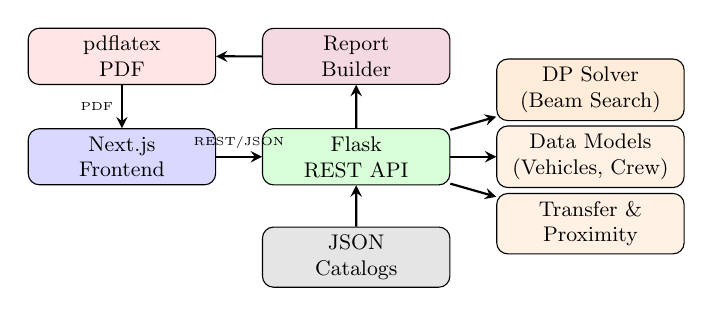
\begin{tikzpicture}[
  box/.style={draw, rounded corners, minimum width=2.8cm,
              minimum height=0.7cm, align=center, font=\small},
  arr/.style={->, >=stealth, thick},
  scale=0.85, transform shape
]
% Frontend box
\node[box, fill=blue!15] (fe) at (0,0) {Next.js\\Frontend};
% API box
\node[box, fill=green!15] (api) at (3.5,0) {Flask\\REST API};
% Solver
\node[box, fill=orange!15] (solver) at (7,1) {DP Solver\\(Beam Search)};
% Models
\node[box, fill=orange!10] (models) at (7,0) {Data Models\\(Vehicles, Crew)};
% Transfer
\node[box, fill=orange!10] (transfer) at (7,-1) {Transfer \&\\Proximity};
% Data
\node[box, fill=gray!20] (data) at (3.5,-1.5) {JSON\\Catalogs};
% Report
\node[box, fill=purple!15] (report) at (3.5,1.5) {Report\\Builder};
% pdflatex
\node[box, fill=red!10] (pdf) at (0,1.5) {pdflatex\\PDF};

\draw[arr] (fe) -- node[above,font=\tiny]{REST/JSON} (api);
\draw[arr] (api) -- (solver);
\draw[arr] (api) -- (models);
\draw[arr] (api) -- (transfer);
\draw[arr] (data) -- (api);
\draw[arr] (api) -- (report);
\draw[arr] (report) -- (pdf);
\draw[arr] (pdf) -- node[left,font=\tiny]{PDF} (fe);
\end{tikzpicture}

  \caption{System architecture. The Flask API exposes five
           endpoints consumed by the Next.js frontend.}
  \label{fig:arch}
\end{figure}

\subsection{Module Catalog}

Fourteen module types spanning six subsystem categories are
defined in the catalog. Table~\ref{tab:modules} lists representative
mass and assembly parameters.

\begin{table}[htbp]
\centering
\caption{Module Catalog (Selected Entries)}
\label{tab:modules}
\begin{tabular}{llrrr}
\toprule
Module & Category & Mass (kg) & Asm.\ Hours & Crew Req. \\
\midrule
Truss Section       & Structural  & 5{,}000  & 48  & No  \\
Habitat Block       & Habitation  & 20{,}000 & 120 & Yes \\
Solar Array Unit    & Power       & 6{,}000  & 36  & No  \\
Fission Reactor     & Power       & 15{,}000 & 100 & Yes \\
Fusion Reactor      & Power       & 40{,}000 & 160 & Yes \\
Chemical (LOX/LH2)  & Propulsion  & 15{,}000 & 80  & Yes \\
NTP Engine          & Propulsion  & 25{,}000 & 120 & Yes \\
NEP Drive           & Propulsion  & 30{,}000 & 160 & Yes \\
SEP Drive           & Propulsion  & 10{,}000 & 100 & Yes \\
Avionics \& Comms   & Avionics    & 4{,}000  & 60  & Yes \\
Shielding Section   & Specialty   & 4{,}000  & 30  & No  \\
Robotic Arm Station & Specialty   & 2{,}500  & 48  & Yes \\
\bottomrule
\end{tabular}
\end{table}

\subsection{Assembly DAG and Parametric Generator}

Module interdependencies are encoded in a directed acyclic graph
(DAG). A parametric generator maps high-level spacecraft
specifications (total length, propulsion type, power type) to a
topologically valid module set. Key ordering rules enforced by the
DAG are: truss sections precede all modules that mount to them;
power systems precede dependent propulsion (NEP requires
Fission/Fusion; SEP requires Solar Arrays); at least one
Airlock/Docking Node must be complete before crew can board.

\subsection{Vehicle Catalog}

Nine cargo launch vehicles, four crew vehicles, and three transfer
stages are cataloged. Table~\ref{tab:vehicles} lists cargo vehicles.

\begin{table}[htbp]
\centering
\caption{Cargo launch vehicle catalog with lead-time and first-flight cost parameters.}
\label{tab:vehicles}
\begin{tabular}{llrrrrl}
\toprule
Vehicle & Nation & LEO (t) & Cost (\$M) & Lead (mo) & $\delta_v$ & Status \\
\midrule
Starship       & USA      & 150 &     100 &  4.1 & 0.20 & Near-term \\
SLS Block 2    & USA      & 130 & 4{,}100 &  6.0 & 0.12 & Operational \\
Falcon Heavy   & USA      &  64 &     150 &  0.9 & 0.08 & Operational \\
New Glenn      & USA      &  45 &      90 &  3.0 & 0.20 & Near-term \\
Vulcan Centaur & USA      &  27 &     130 &  1.8 & 0.08 & Operational \\
Ariane 6       & Europe   &  22 &     110 &  3.0 & 0.10 & Operational \\
KSLV-III       & S.~Korea &  10 &      80 & 18.0 & 0.40 & In dev. \\
GSLV Mk III    & India    &  10 &      50 &  3.0 & 0.10 & Operational \\
H3             & Japan    &   7 &      50 &  3.0 & 0.10 & Operational \\
\bottomrule
\multicolumn{7}{l}{\small Lead time in calendar months (= periods $\times$ 7\,days / 30).
  $\delta_v$ = first-flight cost premium (Eq.~\ref{eq:firstflight}).}
\end{tabular}
\end{table}

\begin{table}[htbp]
\centering
\caption{Crew vehicle catalog. Costs are per mission (vehicle + launch vehicle combined).
  Crew Dragon and Starliner derived from NASA CCtCap per-seat pricing;
  Orion reflects capsule production cost excluding SLS; Starship HLS is SpaceX aspirational production rate.}
\label{tab:crew_vehicles}
\begin{tabular}{llrrrrl}
\toprule
Vehicle      & Nation   & Crew & Cost (\$M) & Lead (mo) & $\delta_v$ & Status \\
\midrule
Crew Dragon  & USA      & 7 &  220 & 1.8 & 0.08 & Operational \\
Starliner    & USA      & 7 &  360 & 3.0 & 0.10 & Operational \\
Orion        & USA/ESA  & 4 &  600 & 6.0 & 0.12 & Operational \\
Starship HLS & USA      & 6 &  250 & 6.0 & 0.20 & Near-term \\
\bottomrule
\multicolumn{7}{l}{\small Lead time in calendar months.
  $\delta_v$ = first-flight cost premium (Eq.~\ref{eq:firstflight}).}
\end{tabular}
\end{table}

\subsection{Web Application}

The Next.js frontend provides: a configuration panel for
spacecraft parametric definition, vehicle selection, objective
weight sliders, and DP solver parameters; a results dashboard
with a Gantt chart, resource utilization charts, cost breakdown,
and 2D assembly progression view; real-time playback controls
with variable speed; and multi-scenario Pareto frontier
visualization. The \texttt{/api/report} endpoint accepts tagged
runs and returns a compiled PDF of this document with
auto-generated results sections.
